\graphicspath{{./images/}}

\chapter{Lösung}

Wie bereits in der Ausgangslage beschrieben wurde für die Lösungsfindung Scrum und Prototyping verwendet. Trotz der iterativen Natur zieht sich ein roter Faden durch den Ablauf der Arbeit. Gewisse Teile wurden gleichzeitig bearbeitet, werden im Text jedoch aufeinanderfolgend beschrieben.

\section{Kontextabgrenzung}

Als erster Schritt musste der Umfang der Arbeit definiert werden. Die Applikation MEON besteht aus mehreren Teilen und benötigt diverse Umsysteme um den Anwendungsfall bereitzustellen. Sämtliche internen Umsysteme wurden deshalb für die Erarbeitung der Lösung nicht berücksichtigt. Diese Systeme sind kritisch für SIX und unterliegen deshalb restriktiven Vorgaben. Die Workflow Engine, welche eigentlich Teil der Applikation ist, wurde ebenfalls ausgeklammert, da es sich um ein Produkt einer externen Firma handelt und deshalb nicht direkt beeinflusst werden kann. Obschon das Produkt mittlerweile Funktionen bereitstellt welche sich mit den Anforderungen decken, ist dafür ein Supportvertrag nötig. Die Entscheidung, ob eine Enterprise Version mit Support gekauft wird, ist noch hängig und wird nicht bis zum Ende der Thesis erwartet.

\section{Anforderungen}

Bevor eine Lösung erarbeitet werden konnte, mussten die Anforderungen an die neue Software Architektur definiert werden. Leider waren die aktuellen Anforderungen ebenfalls nicht in schriftlicher Form vorhanden wodurch diese zusätzlich erfasst werden mussten. Da die Funktionen der Applikation hauptsächlich durch die Software Entwicklung getrieben wurden, konnte der Product Owner des Projektes direkt zu den Anforderungen befragt werden. Bei der Ausarbeitung der Anforderungen hat sich gezeigt, dass die Applikation funktional unverändert bleibt und der Schwerpunkt auf den nicht funktionalen Anforderungen liegt. Durch die Problemstellung resultiert daraus die Hauptanforderung, dass der Benutzer von einer Aktualisierung der Anwendung nichts merkt und dadurch der Dienst selber verfügbar bleibt. Aufgrund von Wartungsarbeiten an Netzwerkkomponenten, Datenbanken, oder an Betriebssystemen kann es dennoch zu Unterbrüchen kommen welche jedoch nicht Gegenstand der Lösung sind. Alle Anforderungen finden sich im SAD im Kapitel 1.3

\section{Qualitätsziele}

Anhand der Anforderungen haben der Product Owner und der Systemverantwortliche mittels des Schemas aus \cite[p.305-311]{esa} die Qualitätsziele in einer ersten Version beschrieben. In einem zweiten Schritt wurden die Ziele zusammen besprochen und angepasst. Vor allem das Ziel bezüglich PCI Compliance erhält eine hohe Gewichtung. Die Applikation selber hält zwar keine relevanten Daten welche unter diese Vorgaben fallen und ist durch die Netzwerksegmentierung getrennt. Durch das hohe Risiko wurde das Szenario dennoch aufgeführt. Sämtliche Ziele und die dazugehörigen Szenarien sind im SAD im Kapitel 10.2 aufgeführt.

\section{Problematik}

Schon während die Anforderungen und Qualitätsziele in der Ausarbeitung waren, musste ein Verständnis für die Probleme, welche sich mit Continuous Deployment ergeben, erworben werden. Als Startpunkt wurde \cite{cd} verwendet. Die Begrifflichkeiten haben sich in der Zwischenzeit geändert und neue Technologien, wie die der Docker Container, erlauben heute andere Lösungsansätze. Daher galt es als erstes zu definieren was Continuous Deployment ist. Um sich ein Bild zu machen wurde dafür mittels Internet Recherche nach dem Begriff gesucht. Eine erste gute Definition fand sich unter \cite{atlassiancd} welche zusätzlich diverse Vorschläge für die Umsetzung enthielt. Auch der Blogeintrag von Thoughtworks \cite{thoughtcd} hatte wertvolle und zeitgemässere Informationen zum Thema. Nach gründlicher Studie der Einträge konnte die generelle Definition auf 'Software jederzeit und ohne Unterbruch des Diensts aktualisieren zu können' festgelegt werden. Für die Umwälzung auf eine Lösung ist die Definition sehr weit gefasst und wird teils verschieden verwendet wie die Internet Recherche gezeigt hat. Ein weiterer Begriff, welcher man im Zusammenhang mit Continuous Deployment antrifft, ist 'Zero Down Time' \footnote{Kann teils als Synonym für Continuous Deployment gesehen werden wobei der Begriff je nach Betrachtungsweise andere Implikationen hat.}. Das Erreichen einer hundertprozentigen Verfügbarkeit kann nicht alleine durch eine passende Software Architektur erreicht werden, da diese immer Abhängigkeiten zu anderen Komponenten wie Betriebssystem, Netzwerk etc. hat. Dafür muss die komplette Infrastruktur dementsprechend ausgelegt werden und auch dann ist der aktuelle Standard 'five nine', was einer Verfügbarkeit von 99.999\%, also einem jährlichen Unterbruch von ungefähr 10 Minuten, entspricht. Dies hat entsprechend hohe Kosten zur Folge welche sich nicht jede Firma leisten kann und auch nicht muss.\newline
Nach dem die Begrifflichkeiten klar waren, musste das generell zu lösende Problem identifiziert werden. Bei der fortlaufenden Aktualisierung von Software gibt es immer einen Zeitpunkt bei welchem mehrere Versionen der Anwendung in Betrieb sind. Das folgende Diagramm veranschaulicht das Problem.

\begin{center}
	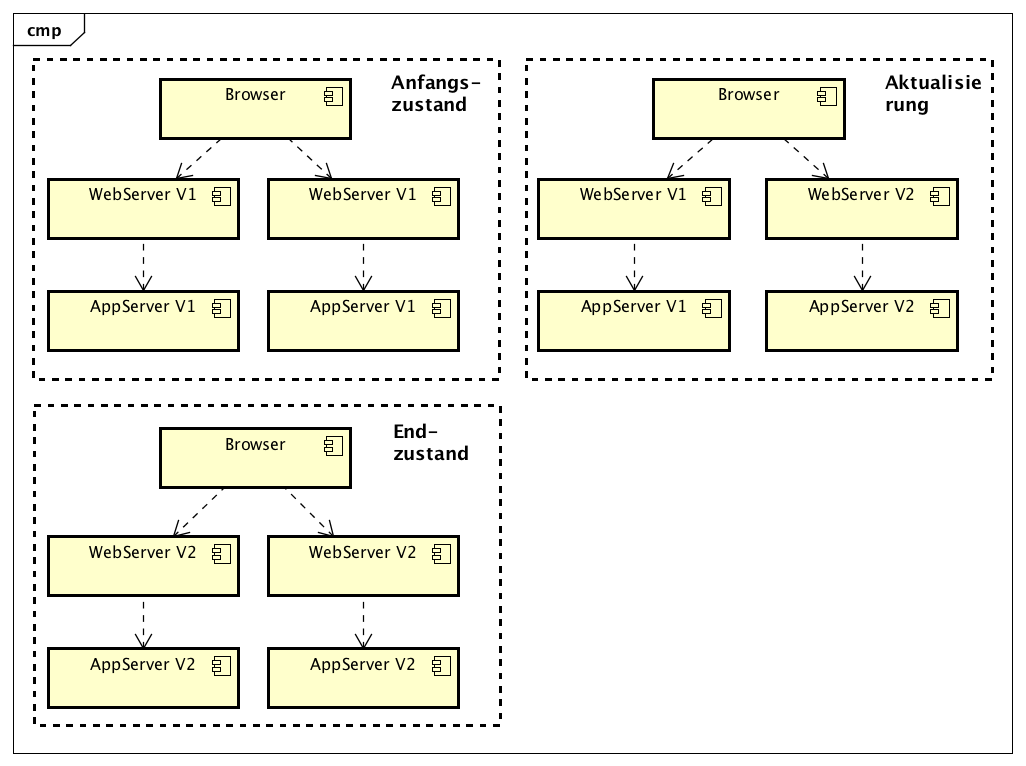
\includegraphics[scale=0.55]{MultiVersion.png}
\end{center}
Daraus lässt sich schliessen, dass die neue Architektur den gleichzeitigen Betrieb von mehreren Versionen unterstützen muss. Dies gilt vor allem für die Schnittstellen und die Datenspeicherung. Da die Applikation nicht geschäftskritisch ist, könnte eine Aktualisierung auch in der Nacht durchgeführt werden wenn sich tendenziell kein Benutzer auf der Webseite befinden. So könnten die Probleme mit der Versionierung der Schnittstelle minimiert werden, für die Datenbank braucht es dennoch eine Lösung.	

\section{Teilprobleme}

Mit dem generellen Verständnis und den Anforderungen konnten nun Teilprobleme identifiziert und nach Lösungsvarianten gesucht werden. Dieses Vorgehen ist in der Arc42 Vorlage nicht explizit ausgewiesen, im Workshop des CAS Software Architektur hat es sich jedoch als hilfreiches Mittel erwiesen das Gesamtproblem in kleinere aufzuteilen und wenn möglich austauschbare Lösungsvarianten zu erarbeiten.

\subsection{Versionierung}

Wie bereits in der Problematik erwähnt, müssen Schnittstellen versioniert werden und abwärtskompatibel sein, damit der Benutzer von einer Änderung nichts merkt. Hier geht es vor allem um die REST\footnote{Steht für Representational State Transfer und ist eine Programmierparadigma welche in verteilten System für die Datenübertragung verwendet wird.} Endpunkte, welche der Onboarding Server der Webseite zur Verfügung stellt.

\subsection{Datenspeicherung}

Ebenfalls in der Problematik erwähnt ist die Datenspeicherung. Aktuell wird für die Applikation eine relationale Datenbank verwendet. Diese Datenbanken haben ein definiertes Schema, welches Datentypen für Felder festlegt und wie die Tabellen miteinander in Beziehung stehen. Hier stellt sich die Frage ob es Lösungen gibt welche den weiteren Einsatz der Technologie erlauben, unter der Berücksichtigung der zusätzlichen Anforderung der Replikation. Soll die Applikation unterbruchsfrei aktualisiert werden können, muss die Datenbank hochverfügbar sein und automatische Mechanismen für den Fehlerfall bereitstellen.

\subsection{Kommunikationsentkopplung}

Soll der Benutzer sich auch bei der Aktualisierung der Applikation für TWINT registrieren können, darf die Anfrage nicht verloren gehen, auch wenn ein Fehler auftritt oder eine Komponente wegen dem Update nicht verfügbar ist. Dies gilt vor allem zwischen Onboarding Server und der Workflow Engine. Obschon diese, wie bereits erwähnt, selbst nicht berücksichtigt wird, sind die Schnittstellen zur Engine davon betroffen.

\subsection{Konfigurationsmanagement}

Aktuell wird das Konfigurationsmanagement mit Hilfe von Docker und Docker Compose bewerkstelligt. Für die neuen Anforderungen muss die aktuelle Lösung geprüft und gegebenenfalls ein anderer Ansatz verfolgt werden. Die Änderung der Konfiguration zur Laufzeit, als neue Anforderung, ist bei einer Applikation die immer wieder ausgerollt werden soll zwingend notwendig um die einzelnen Funktionen besser steuern zu können.

\subsection{Deployment Pipeline}

Die Build Pipeline\footnote{Eine Pipeline ist eine Abfolge von Buildäufträgen(Stages) welche parallel und sequenziell ablaufen können. }, welche im Antrag erwähnt wurde auf Grund ihrer Wichtigkeit für das Bauen und Installieren der Applikation, wurde nicht weiterverfolgt. Der Grund dafür liegt in dem Fortschritt der Methodik, welche das Projekt seit dem Antrag gemacht hat. Wie in \cite{atlassiancd} beschrieben, sind verschieden Stages in der Pipeline sowie Feature Branchens in GIT eine Voraussetzung um eine Applikation zeitnahe in Betrieb zu bringen. Diese Praktiken werden aktuell im normalen Arbeitstag verwendet und müssen deshalb nicht nochmals evaluiert werden.

\subsection{Fazit}

Eine Aufteilung der Problematik in Teilprobleme hat geholfen ein bessere Verständnis zu erlangen welche Aspekte der aktuellen Architektur betroffen sind. Dadurch war eine bessere Fokusierung auf die Variantenfindung möglich und hat verhindert, dass Zeit mit nicht relevanten Themen verschwendet wurde.

\section{Bewertungskriterien}

Die auszuarbeitenden Lösungsvarianten mussten auf ihre Verwendbarkeit geprüft und bewertet werden. Obschon Qualitätsziele für die Architektur definiert sind, eignen sie sich für die Bewertung von Bibliotheken und Lösungsvarianten nur bedingt. Weder das Arc42 Template noch \cite{esa} haben angemessen Metriken und Methoden im Angebot. Aus diesem Grund wurde eine Bewertungsmatrix erstellt welche im CAS Software Architektur Workshop Modul bereits angewendet wurde. Dabei sind die einzelnen Kriterien mit dem Product Owner abgesprochen und gewichtet worden. Der Fokus lag auf Eigenschaften der einzelnen Bibliotheken und Produkte wie Maturität, vorhandenes Wissen, oder potentieller Aufwand für Neuentwicklung und Anpassung. Die Kriterien überlappten sich an einigen Stellen mit den Qualitätszielen, was jedoch nicht als Nachteil gewertet wurde. Die Kriterien sind gezielt vor der Lösungsfindung erstellt worden um den Prozess möglichst objektiv zu halten. Spätere Anpassungen mussten trotzdem gemacht werden da nicht alles von Beginn an klar war. Die Kriterien sind im SAD im Kapitel 9.2 detailliert aufgeführt.

\subsection{Fazit}

Das Erstellen der Bewertungskriterien vor dem Ausarbeiten der Lösungsvarianten hatte den Vorteil, dass die Bewertungen nicht den Lösungen angepasst wurde. Der Nachteil war, dass Kriterien vergessen gingen und teilweise auch erst durch die Prototypen sichtbar wurden. Dadurch mussten eine zweite Bewertungsrunde durchgeführt werden.


\section{Teillösungensvarianten}

Mit den definierten Kriterien sollten verschiedene Varianten für die einzelnen Teilprobleme gesucht werden. Dabei war das Ziel den Lösungsraum möglichst gross zu gestalten um die verschiedenen Ansätze aus verschiedenen Betrachtungsweisen bewerten zu können. Die Ausarbeitung wurde mittels Internet Recherche zu den einzelnen Themen durchgeführt, wobei noch keine technische Prototypen erstellt worden sind. Für alle Varianten wurden Vor-, Nachteile sowie Risiken erfasst und festgehalten. Sämtliche Details zu den Varianten finden sich im SAD im Kapitel 9.1.

\subsection{Versionierung}

Damit die Schnittstellen mehrere Versionen anbieten können, muss ein Weg gefunden werden dies in einer Art zu definieren. \newline Eine erste Variante ist die URL mit einer Versionsvariable zu versehen. Dadurch kann der Client den passenden Endpunkt ansprechen welche die gewünschte Funktionalität bereitstellt. Dies ist ein Standardansatz welcher oft verwendet wird. Die zweite Möglichkeit ist die in \cite{contneg} beschriebene Variante. Dabei wird mittels des Accept-Headers im HTTP-Request die Version mitgegeben. Diese kann auf der REST Schnittstelle als Routinginformation verwendet werden um den Aufruf an eine bestimmte Methode weiterzuleiten. Dieser Ansatz ist ebenfalls ein gängiges Mittel um einen Endpunkt zu versionieren. Als letzte Variante wäre die Verwendung der \cite{gq} Bibliothek, welche von Facebook entwickelt wurde, um das Problem mit verschiedenen Client Versionen zu lösen. Es gibt mehrere Implementation von GraphQL für diverse Sprachen, darunter JavaScript und Java, welche im Projekt verwendet wurden. Die Library wird in einem anderen Projekt bei SIX, welches vom gleichen Team entwickelt wird wie MEON, bereits eingesetzt.

\subsection{Datenspeicherung}

\subsubsection{CAP-Theorem}
Die Anforderungen an die Applikation fordern, dass für die Datenspeicherung Replikation verwendet wird. Im Zusammenhang von verteilten System hört man immer wieder vom CAP-Theorem welches 1998 von Eric Brewer definiert wurde. Es besagt, dass Systeme nur zwei der drei Eigenschaften, Konsistenz, Verfügbarkeit und Partitions Toleranz haben können. Das Theorem wurde vor allem durch die NoSQL Datenbanken wieder aktuell, da diese auf andere Weise funktionieren wie relationale Datenbanken. Die folgende Grafik zeigt wie die Datenbanken kategorisiert sind.
\begin{center}
	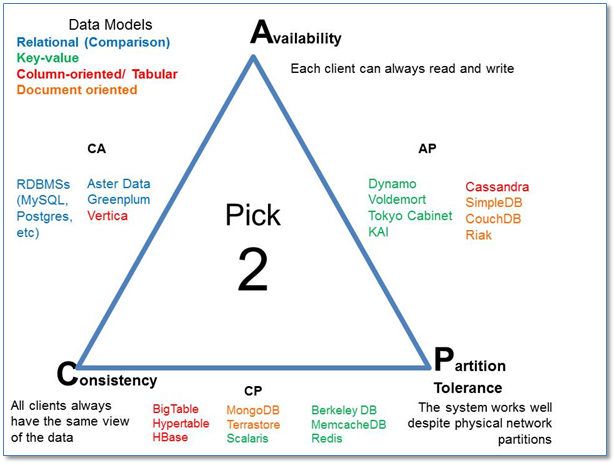
\includegraphics[scale=0.60]{cap.png}\newline
	\cite{cap}
\end{center}
Für einfache Kategorisierung ist diese Grafik hilfreich, jedoch hat sich die Technologie in der Zwischenzeit weiterentwickelt, was Eric Brewer selber in \cite{capnew} mit diversen Beispielen beschreibt. Gewisse Produkte, welche auf dem Markt sind, lassen sich je nach Bedarf anders konfigurieren und können so andere Eigenschaften annehmen. Ein Beispiel hierfür ist die Oracle Datenbank. Oracle RAC zielt auf Verfügbarkeit und Konsistenz und hat entsprechende Anforderungen an die Hardware. Es gibt aber auch die Möglichkeit die Replikation asynchron zu konfigurieren, wodurch sich die Eigenschaften nach Konsistenz und Paritions Toleranz verschieben. 

\subsubsection{Varianten}
Bei der Datenspeicherung war die Frage ob der aktuelle Ansatz mit einer relationalen Datenbank der richtige Weg ist oder ob sich die neuen schemalosen NoSQL Datenbank für die Lösung des Problems besser eignen.\newline
Bei SIX wird Oracle seit langer Zeit eingesetzt und ist der Standard für Datenspeicherung jeglicher Art. Aus diesem Grund wurde dies logischerweise als Variante in Betracht gezogen. Sie bietet alle Features um Anwendungen im Geschäftsbereich zu betreiben.\newline
Die zweite Variante in der Liste ist die MySQL Datenbank. Diese wird aktuell in der produktiven Applikation verwendet was sie ebenfalls als Kandidaten für die Speicherung der Daten empfiehlt.
MySQL bietet wie Oracle diverse Mechanismen welche für Geschäftsanwendungen unumgänglich sind. Das Know-how für den Betrieb ist jedoch nicht auf dem gleichen Stand wie bei Oracle.\newline
Eine neue Möglichkeit der Datenspeicherung sind NoSQL\footnote{NoSQL steht für Not Only SQL und kategorisiert Datenbanken welche schemalos sind und nicht nach dem ACID Prinzip arbeiten.} Datenbanken. Die Idee für deren Verwendung stammt vom CAS Big Data und den dazu gehörenden Folien \cite{nosqlintro}. Daraus ergab sich die dritte Variante die Speicherung mit MongoDB zu realisieren. Die Datenbank arbeiten im Unterschied zu relationalen Datenbanken nicht mit Tabellen sondern mit Dokumenten. Diese sind schemalos und können deshalb gleichzeitig in mehreren Versionen vorliegen. Dadurch ist bei einem Update der Anwendung keine Schemamigration notwendig.\newline
Als letzte Variante wurde Redis in Betracht gezogen. Es handelt sich dabei ebenfalls um eine NoSQL Datenbank welche jedoch ein Key-Value Store ist. Sie verfügt über eine Abfrage Sprache um Daten zu finden und wird auch bereits bei SIX verwendet. Im Bereicht der NoSQL Datenbanken gibt es noch zwei weitere Typen, Kolonnen und Graphen. Diese Varianten wurden nicht berücksichtigt weil sie nicht zum Anwendungsfall passen.

\subsection{Kommunikationsentkopplung}

Damit Anfragen nicht verloren gehen, muss eine Art der Zwischenspeicherung oder der asynchronen Kommunikation gefunden werden. In der Java Welt existieren diverse Technologien dies zu erreichen.\newline
Die Entkopplung zwischen dem Onboarding Server und der Workflow Engine könnte via JMS erreicht werden. Hierzu wird auf dem Server eine Queue angelegt welche auf dem Dateisystem gespeichert und vor der Workflow Engine regelmässig abgefragt wird. Eine Option wäre die zentrale Messaging Infrastruktur der SIX zu verwendent. JMS wird in diversen Projekten verwendet und ist deshalb in seiner Verwendung bekannt.\newline
Im CAS Big Data wurde Kafka vorgestellt welche als weitere Lösung in Betracht kommt. Ursprünglich bei LinkedIn entwickelt, wurde der Source Code 2011 veröffentlicht und wird mittlerweile von der Apache Foundation verwaltet. Kafka wurde für High Performance Messaging entwickelt und ist bei diversen anderen Internetfirmen in Betrieb.\newline
Eine weitere Variante ist die Verwendung von Redis als Queue für die Kommunikation. Die Datenbank hat spezifische Kommandos für die Funktion wie in \cite{redisqueue} beschrieben. Da sie ebenfalls als Datenspeicher eine Variante ist, könnten hier Synergien genutzt werden.\newline
Anstelle eines neuen Frameworks oder einer neuen Technologie könnte die aktuelle Implementation mit Spring Rest und Hystrix weiterverwendet werden. Hierfür bräuchte es eine Art Zwischenspeicher für die Anfragen damit diese asynchron weiter geschickt werden könnten. Die verwendete Datenbank könnte diese Aufgabe übernehmen und würde dadurch zur Queue werden.

\subsection{Konfigurationsmanagement}

Als letztes Teilproblem ist das Verwalten der Konfiguration der Applikation. Mit Docker und Docker Compose sind bereits Tools in Betrieb welche Konfigurationsmanagement erlauben. Als Zusatz käme Docker Swarm zum Einsatz welches es die dynamische Skalierung der Applikation erlaubt.\newline
OpenShift ist ein Produkt der Firma Red Hat welche auf dem Kubernetes Framework von Google basiert. Es handelt sich dabei um eine Plattform as a Service\footnote{Plattform as a Service, kurz PaaS, ist eine Art Cloud dienst, welcher lokal oder remote, bezogen werden kann. Dabei soll eine einheitliche Plattform für alle Anwendungen bereitgestellt werden damit die Entwicklung und der Betrieb nicht immer das ganze Setup für eine Applikation machen müssen.} welche die Infrastruktur für Docker Container bereitstellt. Die bereits vorhandenen Container könnten dabei wiederverwendet werden.\newline
Spring Cloud Config, als weitere Variante, bietet die Möglichkeit Konfigurationen einer Applikation zur Laufzeit anzupassen. Dabei werden die Einstellungen in einem GIT Repository gespeichert und vom Config Server ausgelesen. Clients laden die Konfiguration beim Start oder dynamisch bei einer Benachrichtigung über eine Queue.
Saltstack als letzte Variante wird aktuell bei SIX für das Konfigurationsmanagement der Linux Server verwendet und ist aktuell das Standard Tool. Saltstack hat dabei einen Master Server welche die Serverdefinitionen in einer Datei abgelegt hat und diese entweder über SSH oder Python Client verteilt.

\subsection{Fazit}

Ein möglichst grosser Lösungsraum an Varianten, wie er durch Recherchen, persönliche und Erfahrungen von Dritten erschaffen wurde, hilft die Ideen mittels verschiedenen Perspektiven zu beleuchten. Dadurch können Vor- und Nachteile besser bewertet werden und verhindern falsche Schlüsse. Die Methode bedarf aber einer gewissen Reife und Kenntnisse diverser Konzepte. Ohne diese Voraussetzung besteht die Gefahr das der Lösungsraum zu klein wird oder man Technologien und Methoden verwendet welche einem am besten vertraut sind.

\section{Erste Bewertung der Varianten}

Nachdem für alle Teilprobleme verschiedene Lösungsvariaten definiert wurden, galt es diese zu bewerten um zu entscheiden für welche Prototypen erstellt werden sollten. Die Bewertung wurde zusammen mit dem Product Owner durchgeführt um eine zu einseitige Bewertung zu verhindern. Dabei wurde vor allem auf persönliche Erfahrung mit Technologien und logische Abschätzung gesetzt. Die Entscheidung einen Prototypen zu erstellen war einerseits die Verifikation ob die Lösungsvariante die Richtige ist respektive um Unklarheiten aus dem Weg zu räumen. Die Bewertungen finden sich in der Datei 'Bewertungsmatrix.xslx'. 

\subsection{Versionierung}

Bei der Versionierung haben sich Content-Negotiation und die Versionierung mittels Pfad als gleichwertig herausgestellt. GraphQL als Variante konnte nur schwer bewertet werden, da der existierende Prototyp nicht wirklich aussagekräftig war. Aus diesem Grund wurde entschieden für GraphQL einen Prototypen zu erstellen um die Angemessenheit zu beweisen.

\subsection{Datenspeicherung}

Die beste Bewertung für die Speicherung der Daten hat Oracle erhalten, da diese durch den langen Einsatz in der Firma bestens bekannt ist. In einem Gespräch mit dem Betrieb kam heraus, dass SIX keine Lizenzen zum Betreiben dieser Datenbank auf der virtuellen Umgebung besitzt. Der Grund hierfür ist das Lizenzmodell von Oracle bei welchem sämtliche CPU Cores der virtuellen Umgebung lizenziert werden müssen. Dies hätte sehr hohe Kosten zur Folge. Im Gespräch kam heraus, dass nur eine physische Maschine in Frage käme. 
De Anforderung der Replikation hätte weitere Kosten zur Folge welche für die wenigen Tabellen der Applikation keinen Sinn ergeben.
Die Variante Redis wurde früh verworfen weil die Funktionsweise der Datenbank nicht sonderlich gut mit der Applikation zusammen passt. Der Grund ist hauptsächliche das Speichermodell von Key-Value.
Durch die Bewertung blieben nur MySQL und MongoDB übrig. Leider konnten für beide die Tauglichkeit bezüglich Replikation und Schemamigration nicht ausreichend beantwortet werden weshalb die Entscheidung für je zwei Prototypen respektive entsprechende Nachforschungen getroffen wurde.

\subsection{Konfigurationsmanagement}

Docker Compose wurde bei einem Interview mit den Entwicklern als ungenügend dokumentiert und schwerfällig bezeichnet, weshalb es als künftige Variante nicht in Frage kommt. Die Docker Container selber wurden als angemessene Lösung empfunden und sollten deshalb, wenn möglich, weiterverwendet werden. Saltstack arbeitet generell mit anderen Konzepten als die jetzt verwendeten Container, was einen Einsatz nicht sinnvoll macht, obschon die Bewertung eher hoch ausgefallen ist. OpenShift, als Variante, hat eine schlechtere Bewertung als SaltStack, ist für die Firma mittlerweile aber von strategischer Bedeutung was Aussagen des Product Owner auch belegen. Daher ist eine Verwendung unumgänglich weil anderenfalls die Lösung unter die Kategorie 'Special Solutions' fällt und die Kosten dadurch selber getragen werden müssen. Für OpenShift mussten jedoch weitere Recherchen gemacht werden um den Einsatz besser abzuschätzen zu können. Die beste Bewertung hat Spring Cloud Config erhalten vor allem wegen des guten Know-hows und der Bekanntheit von Spring. Nichtsdestotrotz wurde entschieden ein Prototypen zu machen um die Funktionsweise verifizieren zu können.

\subsection{Kommunikationsentkopplung}

Die Bewertung der Entkopplung wurde in einem ersten Durchgang ausgelassen, da zu dieser Zeit das Team, welches die Applikation betreut, Änderungen an diesem Teil implementierte. In Absprache mit dem Product Owner wurde diese Entscheidung deshalb zurückgestellt.

\subsection{Fazit}

Eine erste Bewertungsrunde hat geholfen die absehbar unpassendsten Lösungen von vornherein auszuschliessen. Es zeigt aber auch, dass die Skalierung und Summe der Ergebnisse teilweise durch die Menge die Resultate verwässern respektive die Skalierung einzelner Kriterien nicht in den Raster passen. Dies ist am Beispiel von Oracle gut zu sehen, hat sie doch die beste Bewertung erhalten, konnte aber aufgrund von Lizenzbestimmungen nicht verwendet werden. Eine frühere Absprache mit dem Datenbankbetrieb hätte diese Problem behoben.

\section{Prototypen}

Mit den erstellten Bewertungen sollten nur die Prototypen umgesetzt werden um in einem zweiten Schritt die Bewertungen für die offenen Punkte abzuschliessen. Weitere Informationen zu den Prototypen finden sich im SAD im Kapitel 9.3

\subsection{MySQL, MongoDB Schema Migration}

Um die Migration des Schemas zu testen, mussten zuerst Use Cases definiert werden welche eine gewisse Komplexität aufweisen um eine sinnvolle Evaluation durchzuführen. Die Wahl fiel dabei auf die zwei folgenden Szenarien:
\begin{itemize}
	\item Änderung einer Spalte
	\item 'Split Table' bei welcher eine Tabelle in mehrere aufgeteilt werden.
\end{itemize}
\newpage
\subsubsection{MySQL}

Das Team, welches bis jetzt die MEON Applikation entwickelt, hatte letztes Jahr ein Kurs zu FlywayDB mit deren Erfinder Axel Fontaine  welcher das Thema Continuous Deployment damals schon ansprach. Er hat dabei auf \cite{rd} verwiesen welche für alle Fälle eine passende Lösung hat. Darin sind die ausgewählten Fälle auf den Seiten 109-113 und 145-151 beschrieben. Das Beispiele Rename Column wurde kurzerhand umgesetzt um zu sehen wie dies bei MySQL funktioniert. Hierfür wird auf den Tabelle die Daten mittels Trigger in die jeweils andere kopiert und so sicher gestellt die Applikation mit verschiedenen Versionen zugreifen kann. Der folgende Codeausschnitt illustriert das Beispiel, welches mit Hilfe von \cite{mysqltrigger} erstellt wurde.

\begin{lstlisting}[language=SQL, showspaces=false, basicstyle=\ttfamily, numbers=left, numberstyle=\tiny, commentstyle=\color{gray}]

DROP TRIGGER IF EXISTS ins_lastname;
DROP TRIGGER IF EXISTS up_lastname;

DELIMITER $$

create trigger ins_lastname BEFORE INSERT on t_person 
	for EACH ROW
	BEGIN
		IF new.last_name is not null then
			set NEW.sur_name = NEW.last_name;
		else
			set NEW.last_name = NEW.sur_name;
		end if;
	END $$

create trigger up_lastname BEFORE UPDATE on t_person
	for EACH ROW
	BEGIN
		IF new.last_name is not null then
			set NEW.sur_name = NEW.last_name;
		else
			set NEW.last_name = NEW.sur_name;
		end if;
	END $$

DELIMITER ;

\end{lstlisting}
Somit hat MySQL die Möglichkeiten welche für das Erfüllen der Ziele notwendig sind.
\newpage
\subsubsection{MongoDB}

Für MongoDB musste zuerst recherchiert was die beste Methode ist um verschiedenen Dokumenteversionen zu verwalten. In \cite{mongoschema} wurde einfach aufgezeigt wie dieses Problem gelöst werden kann. Dokumente werden mit einem Attribut für die Version versehen, welches durch die Entwicklung angehoben wird falls Änderungen gemacht wurden. Des weiteren werden Felder nicht gleich gelöscht sondern 'Deprecated' markiert und erst zu einem späteren Zeitpunkt entfernt. Um den Prototypen zu verifizieren wurde eine kleine Spring Boot Applikation geschrieben, welche unter \url{https://github.com/effusion/prototyps/tree/master/springmongo} zu finden ist. Dabei wurden zwei Branches erstellt und entsprechende Docker Images gebaut. Dadurch konnten zwei Versionen der Applikation laufen und gleichzeitig auf die Datenbank zugegriffen werden. 
Eine Abfrage auf der Datenbank liefert folgendes Resultat.


\lstset{
	string=[s]{"}{"},
	stringstyle=\color{blue},
	comment=[l]{:},
	commentstyle=\color{black},
}
\begin{lstlisting}
{
	"_id" : ObjectId("586bee9446e0fb000606b7c4"),
	"_class" : "ch.andreas.thesis.mongo.data.Person",
	"documentVersion" : NumberLong(1),
	"surName" : "Heubeck",
	"firstName" : "Anita",
	"streetName" : "Riedweg",
	"houseNumber" : 14,
	"town" : "Dübendorf",
	"zip" : 8600,
	"country" : "Schweiz"
	},
	{
	"_id" : ObjectId("586c09229d669165fd903240"),
	"_class" : "ch.andreas.thesis.mongo.data.Person",
	"documentVersion" : NumberLong(2),
	"surName" : "Heubeck",
	"firstName" : "Anita",
	"addressList" : [
	{
		"documentVersion" : NumberLong(1),
		"streetName" : "Riedweg",
		"houseNumber" : 14,
		"town" : "Dübendorf",
		"zip" : 8600,
		"country" : "Schweiz"
	}	
	],
	"houseNumber" : 0,
	"zip" : 0
}
\end{lstlisting}
Im Resultat ist ersichtlich, dass zwei Versionen des Dokuments in der Datenbank gespeichert wurden. Die Applikation muss die Daten dann passend für die Version über die REST Schnittstelle konvertieren. Auch MongoDB kann mit diesem Beweis die Anforderungen erfüllen.

\subsection{MySQL, MongoDB Replikation}

\subsubsection{MySQL}

Die Datenbank wird aktuell schon mit einem Master-Slave Verfahren betrieben hat aber keinen automatischen Failover und eine Anpassung der Verbindung in der Applikation ist ebenfalls nötig. Die Recherche hat ergeben, dass es eine Möglichkeit gibt die Umschaltung automatisch zu machen wie im Artikel \cite{mysqlrep} beschrieben. Dabei wird ein separates Programm installiert, welche die einzelnen Instanzen überprüft und neu startet. Damit die Applikation nicht neu gestartet werden muss kann der Datenbankverbindung, wie in der Anleitung \cite{mysqljdbc} beschrieben, konfiguriert werden. Für MySQL gibt es noch eine weitere Replikationsvariante mit einem Cluster wie in \cite{mysqlcluster} beschrieben. Dies wurde aufgrund mangelnden Wissens auch Seitens des Betriebs nicht berücksichtigt. Die Recherchen sind gemäss Ansichten des Product Owners ausreichend um zu beweisen, dass MySQL die Anforderungen erfüllt.

\subsubsection{MongoDB}

Da MongoDB noch nicht im Einsatz war wurde auch hier eine Recherche zu Replikationsmöglichkeiten gemacht. Die Datenbank hat in der Anleitung ein Kapitel \cite{mongorep} welches die genaue Konfiguration beschreibt. Im Vergleich zu MySQL gibt es wenig Know-How für MongoDB zur Replikation. Deshalb wurde neben den offiziellen Quellen eine einfache Anleitung gesucht und mit \cite{mongorep2} auf gefunden. Das Tutorial ist simpel gehalten ermöglichte aber die einfache Verifikation der Replikationsfähigkeiten von MongoDB und damit die Erfüllung der Anforderungen.
\newpage

\subsection{GraphQL}

Um GraphQL besser verifizieren zu können, wurden ebenfalls einige Anwendungsfälle mittels eines einfachen Prototypen umgesetzt. Der Source Code dazu findet sich unter \url{https://github.com/effusion/prototyps/tree/master/graphql}. Die Use Cases wurden in JUnit definiert und gegen das erstellte GraphQL Schema getestet, welches mit Hilfe der Beispiele von \url{https://github.com/graphql-java/graphql-java/blob/master/src/test/groovy/graphql/StarWarsSchema.java} erstellt wurde. Dabei hat sich herausgestellt, dass vor allem die Konvertierung der Daten beim Schreiben einen hohen Aufwand und viel Typen Casting benötigt. Je verschachtelter die Datenstruktur ist, desto mehr muss auch für die Konvertierung gemacht werden. Dies kann durch eine geschickte Definition der REST Schnittstelle teilweise kompensiert werden, verschiebt das Problem jedoch nur. Der folgende Codeauschnitt zeigt die Problematik:

\begin{lstlisting}[language=Java, showspaces=false, basicstyle=\ttfamily, numbers=left, numberstyle=\tiny, commentstyle=\color{gray}]
/*Converter methods to fetch all the data out of the map*/
private Object addPerson(Map<String, Object> envMap) {
	Person person = new Person();
	person.setFirstName( (String) envMap.get("firstName"));
	person.setLastName( (String) envMap.get("lastName"));
	convertAddress(person,(ArrayList<Object>) envMap.get("newAddresses"));
	personRepository.createPerson(person);
	return person;
}

	private void convertAddress(Person person, ArrayList<Object> newAddresses) {
	final List<Address> addressList = new ArrayList<>();
	newAddresses.forEach(entry -> {
		LinkedHashMap<Object,Object> addressAttributes = (LinkedHashMap<Object,Object>) entry;
		createAddress(addressList, addressAttributes);
	});
	person.setAddresses(addressList);
}

private void createAddress(List<Address> addressList, LinkedHashMap<Object,Object> addressAttributes) {
	Address address = new Address();
	address.setStreetName((String) addressAttributes.get("streetName"));
	address.setHouseNumber((long) addressAttributes.get("houseNumber"));
	address.setTown((String) addressAttributes.get("town"));
	addressList.add(address);
}
\end{lstlisting}
GraphQL kommt ursprünglich aus der Welt der dynamischen Sprachen wo die Konvertierungen nicht gemacht werden müssen. Der Prototyp hat gezeigt, dass die Bibliothek die Anforderungen zwar erfüllen würde, die Umsetzung jedoch zu umständlich ist.

\subsection{Spring Cloud Config}

Um die Verwendbarkeit von Spring Cloud Config zu evaluieren wurde wiederum ein Prototyp mit einem Client und einem Server gemacht. Der Sourcecode findet sich unter \url{https://github.com/effusion/prototyps/tree/master/springconfig}. Der Prototyp wurde mit Hilfe von dem Getting Started Guide \cite{gsspringcloudconfig} umgesetzt. Diesem fehlte jedoch noch die Komponente der automatischen Verteilung der Konfigurationen bei einer Änderung. Durch weitere Internet Recherchen konnte ein Tutorial \cite{springcloudpush} eines Pivotal Mitarbeiters gefunden werden, welches genau diesen Teil erklärt. Nach Anpassung des Prototypen funktionierte auch die Benachrichtigung.
Das Framework kann die geforderte Anforderungen somit erfüllen.

\subsection{OpenShift}

Um einen ersten Eindruck von OpenShift zu gewinnen, musste zuerst das Konzept der Plattform verstanden werden. Mit der neuen OpenShift Version 3 wurde die Plattform auf Basis von Docker und Kubernetes faktisch neu implementiert. Der Startpunkt war \cite{openshiftintro} welches die Grundkonzepte genauer erklärte. Mit diesem Verständnis konnten erste Gehversuche mit der Online Preview für Entwickler gemacht werden. Einfache Container wie MongoDB oder auch Applikationsserver zu starten und miteinander zu verbinden war dank der Templates, welche bereits auf der Plattform verfügbar sind, ohne Probleme zu bewältigen. Eigene Container auf der Umgebung zu deployen hat dann schon einiges mehr Mühe bereitet, vor allem da die Templates in yaml Format voller Parameter sind, welche zu erst verstanden werden müssen. Da SIX intern bereits eine Plattform aufgebaut hat, war der nächste logische Schritt die Administratoren zu kontaktieren. In einem ersten Meeting konnten Verständnislücken geschlossen und eine erste Idee für das Deployment auf OpenShift entwickelt werden. Mitte Januar war ein Solution Architekt von Red Hat zu Schulungszwecken bei SIX, welcher bei einem Meeting ebenfalls wertvolle Tipps geben konnten. Zu diesem Zeitpunkt war klar, dass die Plattform die Anforderungen erfüllen kann.

\subsection{Fazit}

Das Erstellen einzelner Prototypen für die Verifikation der ausgewählten Varianten hat sich als richtiges Mittel erwiesen um die getroffenen Entscheidungen zu verifizieren respektive Annahmen zu widerlegen. Durch die daraus gewonnen Erkenntnisse konnte eine revidierte Bewertung gemacht werden.

\newpage

\section{Finale Bewertung der Varianten}

Nach Abschluss sämtlicher Prototypen und mit den gefundenen Antworten konnte nun die abschliessende Bewertung durchgeführt werden. Für die Punkte der Datenspeicherung mussten noch zwei weitere Bewertungskriterien hinzugefügt werden, welche erst mit der Evaluation aufgefallen sind. Wie bereits beim ersten Durchgang wurden die Bewertungen erneut mit dem Product Owner besprochen. Sämtliche Entwurfsentscheidungen finden sich im SAD im Kapitel 9.4

\subsection{Datenspeicherung}

Beide Varianten, MySQL und MongoDB, konnten die Anforderungen erfüllen. SIX hat mit NoSQL Datenbank aus Betriebssicht wenig Erfahrung weshalb in einem Meeting mit der Datenbankabteilung die Lösungsvariante besprochen wurde. Durch die hohe Auslastung und das aktuelle Thema Database as a Service hat der Betrieb in der Schweiz wenig Möglichkeiten und Kapazitäten die Datenbank zu betreiben. Durch diverse Initiativen innerhalb von SIX sind die involvierten Personen jedoch daran interessiert sich auch in diesen Themen Know-how anzueignen und Unterstützung zu liefern. Dank internen Kontakte konnte ausserdem in Erfahrung gebracht werden, dass SIX USA MongoDB bereits produktiv verwendet. Der Onboarding Server braucht aktuell nur wenige Tabellen, was das Risiko senkt und mit Blick auf die DevOps Initiative wurde die Entscheidung zu Gunsten von MongoDB getroffen.

\subsection{Kommunikationsentkopplung}

Die bei der ersten Iteration zurückgestellte Bewertung konnte, nach Abschluss der Arbeiten, nun gemacht werden. Die Kommunikation ist mittlerweile asynchron, jedoch verwendet sie dafür die Datenbank als Queue und verschickt die Anfragen mit einem Scheduler regelmässig an die Workflow Engine. Aus diesem Grund wurde die Variante mit Spring REST und Hystrix ausgewählt.

\subsection{Fazit}

Durch das Wissen der Prototypen war es folgerichtig die Bewertung nochmals zu besprechen um sich für eine Variante zu entscheiden. Nur durch Recherchen eine Entscheidung zu treffen hätte zu einem späteren Zeitpunkt zu Probleme führen können. Vor allem mit dem Blick auf die neuen Technologien und Methoden welche verwendet werden.

\section{Software Architektur Dokument}

Das Software Architektur Dokument wurde schon während den Evaluationen und dem Prototyping mit den Ergebnissen befüllt. Diese Information sind für eine eventuelle spätere Anpassung der Architektur sehr wichtig um die Entscheidungsvorgänge und Abwägungen, welche getroffen wurden, zu verstehen. Die Applikation ist aktuell in Betrieb und hat auch eine Architektur welche leider sehr knapp dokumentiert ist. Der generelle Aufbau der Applikation war durch die Vorarbeiten für den Antrag bekannt und musste nun mit den restlichen Teilen kombiniert werden. Die ständige Kommunikation mit dem Verantwortlichen der Applikation hat dazu beigetragen, dass keine Überraschungen zu Tage traten.

\subsection{Bausteinsicht}

Von Vorarbeiten her war bekannt, dass die Applikation mit einer Schichtenarchitektur umgesetzt wurde und wie die Schichten auf die einzelnen Komponenten verteilt sind. Der interne Aufbau war hingegen nicht bekannt und musste deshalb zuerst herausgefunden werden. Hierfür wurde einerseits der Sourcecode verwendet und andererseits die beteiligten Entwickler direkt befragt. Eine Schwierigkeit war es die Komponenten der Ebene entsprechend zu kategorisieren und zusammenzufassen. Zusätzlich musste der neue Teil mit der Konfiguration vermerkt werden. Um die Übersicht auf der ersten Ebene zu wahren, wurden auf der zweiten Ebene die wichtigsten Teile genauer ausgearbeitet und mit den Entwicklern verifiziert. Auf eine noch genauere Ebene wurde verzichtet, da die gelieferten Informationen die wichtigsten Aspekte beschreiben. Die Bausteinsicht befindet sich im SAD im Kapitel 6.

\subsection{Laufzeitsicht}

Wie bereits bei der Bausteinsicht, musste auch die Laufzeitsicht nachdokumentiert werden. Der Geschäftsfall war vom Ablauf her klar, nicht jedoch wie die einzelnen Systeme daran beteiligt waren. Um die Informationen zu bekommen, mussten wieder die Entwickler befragt werden, da der Ablauf schwieriger aus dem Sourcecode herauszulesen war. Diese Informationen wurden dann in der ersten Ebene der Sicht aufgezeichnet. Diese war aber noch zu generell weshalb ein weiteres Sequenzdiagramm gezeichnet wurde, welches die Komponenten der einzelnen Schichten enthält. Die Laufzeitsicht für die Registrierung konnte nicht alle Aspekte darstellen weshalb zusätzlich, erneut durch Befragung, ein Aktivitätsdiagramm erstellt wurde. Damit konnte eine komplette Sicht auf den Prozess des Registrierens gewonnen werden.\newline\newline
Durch die Verwendung von Spring Cloud Config ist der Ablauf der Konfigurationsänderung hinzugekommen. Der Prozess ist durch die gute Abstraktion seitens der Bibliothek sehr einfach zu verstehen und benötigt vom Entwickler keinen Programmieraufwand, sondern beschränkt sich auf die Konfiguration. Die Laufzeitsicht befindet sich im SAD im Kapitel 7.

\subsection{Verteilungssicht}

Mit dem Entscheid OpenShift als Plattform zu verwendet anstelle von Docker Compose, musste die Art wie die Applikation verteilt wird neu definiert werden. Vor allem musste Klarheit über die einzelnen Komponenten von OpenShift sowie das Deployment der Plattform selber verstanden werden. Durch SIX interne Kurse mit Red Hat sowie in enger Absprache mit den Administratoren konnte eine erste Idee gewonnen werden. Aktuell ist das Ziel die Plattform in beiden Rechenzentren in Zürich und Lupfig zu installieren und dies jeweils in den Firewallzonen DMZ und PCI. Die Applikation selber weiss nicht wo die einzelnen Teile laufen, sondern überlässt das ganze Routing OpenShift, welches im Endeffekt ein Software Defined Network\footnote{Ein Software Defined Network oder kurz SDN ist eine Technik mit der sich Netzwerktopologien mittels Software definieren und steuern lassen. Somit ist es nicht mehr nötig die Netzwerkkomponenten von Hand zu konfigurieren. } ist. Mit diesem Wissen konnte die Verteilungssicht erstellt und beschrieben werden. Mit OpenShift kommen zusätzliche neue Begriffe hinzu welche angemessen erklärt werden mussten. Diese wurde direkt aus der Dokumentation von \cite{osservicepod} extrahiert. Die Bausteinsicht befindet sich im SAD im Kapitel 8.

\subsection{Konzepte}

Die einzelnen Komponenten der Architektur verwenden verschiedene Konzepte welche für das Verständnis wichtig sind. Die bereits bekannten Konzepte wurden wiederum durch Befragung mit den Entwicklern nach dokumentiert. Das Vorgehen für die neuen Konzepte wird in den folgenden Kapiteln erläutert. Sämtliche Konzepte welche für die Architektur verwendet werden, sind im SAD im Kapitel 9 erklärt.

\subsubsection{Software Aktualisierung}

Mit dem Umbau der Architektur in Richtung kontinuierliche Aktualisierung ist das dahinter stehende Konzept, wie der Entwickler Änderungen macht, integraler Bestandteil. Aus diesem Grund wurde das Kapitel früh im Dokument aufgeführt und mit den wichtigsten Regeln versehen. Die Schnittstellen und die Persistenz sind von der Methode stark betroffen weshalb ein Beispiel eingefügt worden ist.

\subsubsection{Build Management}

Wie die Software gebaut wird, ist meistens nicht Teil eine Software Architektur und wenn dann höchstens die verwendeten Tools. Im Bezug auf Continuous Deployment ist es wichtig, dass der Entwickler nicht nur die Architektur versteht sondern ebenfalls wie die Applikation ausgerollt wird. Mit dem Einsatz von OpenShift ändert sich die Art der Installation welche an Komplexität zugenommen hat.

\subsubsection{Konfiguration}

Durch den kombinierten Einsatz von OpenShift und Spring Cloud Config hat sich die Art wie die Applikation konfiguriert wird geändert. Der Entwickler muss deshalb wissen wo welche Konfigurationen gemacht werden müssen.

\subsubsection{Persistenz}

Mit der Verwendung von MongoDB für die Speicherung der Daten auf dem Onboarding Server, braucht es eine Erklärung wie der neue Datenspeicher funktioniert. Einerseits galt es zu erklären was der Unterschied zwischen Tabellen und Dokumenten ist als auch ein Verständnis dafür wie diese definiert werden müssen. Durch die andere Art der Speicherung gibt es mehrere Möglichkeiten wie die Daten und Beziehungen dazwischen gemacht werden können. MongoDB hat für diesen Fall eine Beitragsreihe \cite{mongoschema1}, \cite{mongoschema2} und \cite{mongoschema3} ins Internet gestellt welche mittels Beispielen die verschiedenen Möglichkeiten aufzeigt.

\subsubsection{Transaktionsbehandlung}

Als letzten Punkt ist es wichtig zu verstehen wie MongoDB mit Transaktionen umgeht und die Daten im Replica Set verteilt werden. Alle Angaben dazu finden sich in der Dokumentation \cite{wirteconcern} und wurden, zum Anwendungsfall passend, beschrieben.

\subsection{Finaler Prototyp}

Die einzelnen Prototypen haben gezeigt, dass die Architektur in der vorgeschlagenen Form umgesetzt werden kann. Da vor allem die OpenShift Plattform für alle Entwickler neu ist, hat man sich entschieden die einzelnen Teilprototypen zu einem End-zu-End Beispiel zusammenzufügen. Dadurch kann ein vertiefter Einblick in Verwendung der Plattform gewonnen und eventuell bis jetzt übersehene Probleme aufgedeckt werden. Dies auch mit dem Hintergrund, dass die Plattform aktuell nur auf Testservern installiert ist und die finale Installation erst gemacht werden muss. Ein weiterer Punkt ist, dass auf höherer Ebene entschieden wurde die ganze MEON Applikation als erste Anwendung produktiv auf OpenShift auszurollen.\newline\newline
Der Prototyp wurde aufgrund des Testserversetups im Vergleich zur Installation, welche im SAD Kapitel 8 beschrieben ist, vereinfacht. Das folgende Darstellung zeigt den Aufbau.

\begin{center}
	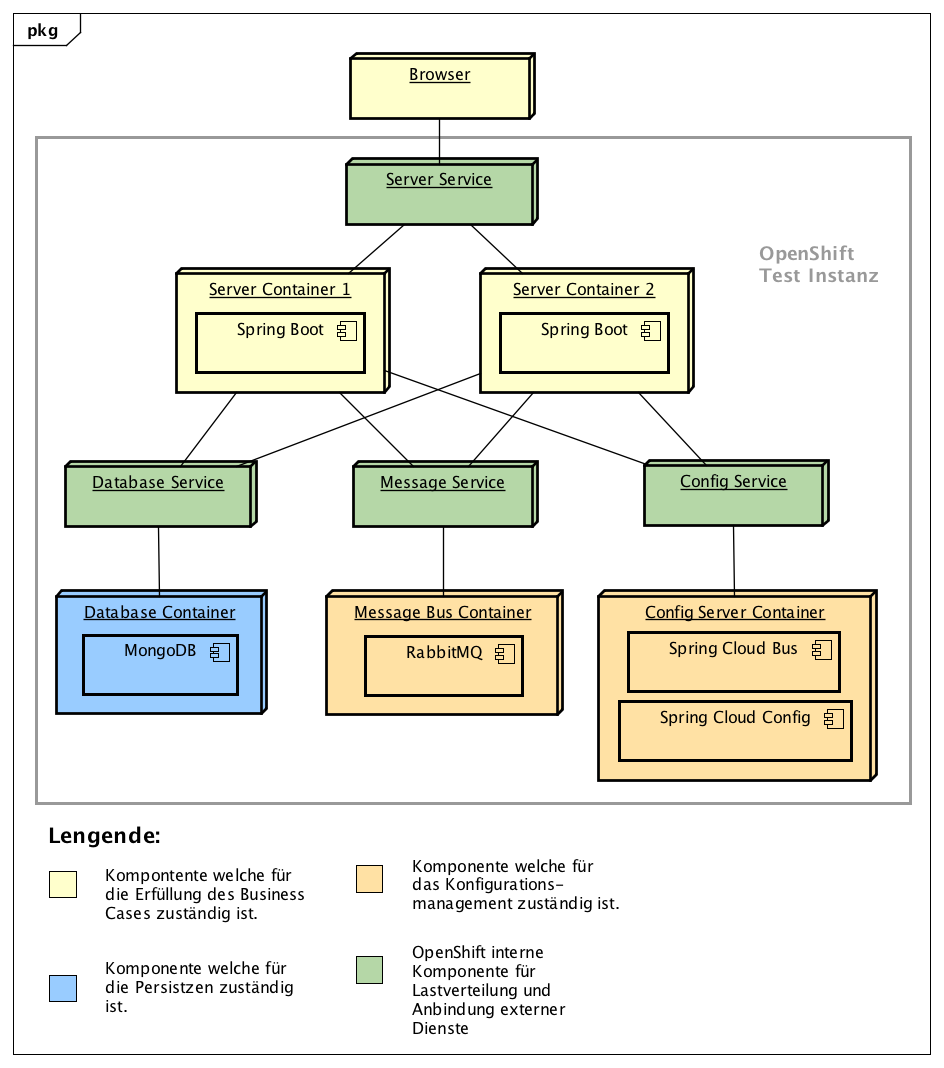
\includegraphics[scale=0.60]{PrototypDeployment.png}
\end{center}

\subsection{Change Management}

{\color{red} Review ganzes Kapitel}
Das Change Management hat durch die vielen Vorschriften und das Umfeld, in welchem SIX tätigt ist, einen wichtigen Stellenwert. Das Change Management war als Stakeholder früh bekannt wurde aber nicht gleich in die Lösung einbezogen da ohne konkrete Ergebnisse eine Demonstration der Möglichkeiten und die damit zusammenhängenden Folgen schwer zu beschreiben waren. Nach dem Abschluss des finalen Prototypen wurde ein Treffen mit dem Change Management abgehalten um das weitere Vorgehen zu besprechen. Folgende Punkte wurden dabei festgestellt:
	
\begin{itemize}
	\item Das ITMS Tool dient nicht nur dem Aufzeichnen von Änderungen sondern ist auch ein Audit Werkzeug.
	\item Anpassungen können schon heute über eine Jira Schnittstelle eingeliefert werden, die Funktionalität ist jedoch noch ausbaufähig.
	\item Continuous Deployment generiert durch die Natur sehr viele Änderungen. Diese würden das System überladen und keinen Nutzen bringen.
	\item SOP's\footnote{Standart Operation Procedures oder Standartvorgehen ist ein definierter Ablauf welcher immer gleich durchgeführt wird.} könnten für die Ausrollung definiert werden da der Prozess automatisch und generell immer gleich abläuft. 
\end{itemize}

Eine vollautomatische Installation ist aktuell auf Grund des Change Managements nicht möglich obschon die Architektur die Möglichkeit hat. Beim Übergang in die Produktion ist ein manueller klickt notwendig. Das Change Management sieht aber auch die Vorteile des Ansatzes benötigt aber einige Zeit um die bestehenden Prozesse anzupassen. 

\subsection{Fazit}

Das Software Architektur Dokument ist ein gutes Mittel und auch Leitfaden um ein System und seine Architektur zu beschreiben. Gernot Starke hat mit dem Arc42 eine gute Basis geschaffen, welche Architekten bei ihrer Arbeit hilft. Es hat sich aber auch gezeigt, dass es sich um ein Grundgerüst handelt, welches stellenweise erweitert werden muss. Das Kapitel Entwurfsentscheidung sei hier erwähnt, da es doch eine detaillierte Beschreibung der getroffenen Entscheidungen zeigt. Ohne diese ist eine spätere Anpassung der Architektur schwierig und mit Aufwand verbunden.
{\color{red} Gibt hier vllt noch Anpassungen nach dem Feedback von Werni}
\newpage
\section{Architektur Bewertung}

Mithilfe des finalen Prototyps konnte die Architektur anhand der Qualitätsziele und Szenarien bewertet werden.

\subsubsection{Ziel: Der Zugriff auf sensitive Daten (PCI) darf nicht möglich sein}

Neben dem schreibenden Zugriff auf die Workflow Engine kommen zwei lesende Zugriffe, auf die Benachrichtigungsqueue und auf den Konfgurationsserver, hinzu. Beide Komponenten haben keinen Zugriff auf Systeme mit Kartendaten. Aus diesem Grund ist das Qualitätsziel erfüllt.

\subsubsection{Ziel: Anpassungen an der Software sollen schnell eingeführt werden können}

Ist die Applikation gebaut, getestet und für den produktiven Betrieb freigegeben, genügt ein Klick oder ein Kommandoaufruf um die Applikation zu installieren. Die OpenShift Container Plattform übernimmt dabei sämtliche weiteren Schritte. Damit ist das Qualitätsziel erfüllt.

\subsubsection{Ziel: Die Applikation soll einfach auf unterschiedlichen Umgebungen installiert werden können}

Die komplette Applikationskonfiguration kann aus OpenShift in ein Template exportiert werden. Dieses Template kann angepasst und später wieder importiert werden. Es gibt auch die Möglichkeit der variablen Konfiguration. Möchte ein Tester oder ein Entwickler die Anwendung testen kann er dieses Template verwendet. Das Ziel gilt generell als erfüllt, eine Umsetzung bedarf jedoch noch eines gewissen Aufwandes um die Vorlagen entsprechend vorzubereiten.

\subsubsection{Ziel: Der Kunde soll bei korrektem Ausfüllen der Daten sich registrieren können}

Durch die Möglichkeit mehrere Instanzen eines Containers zu betreiben, die Funktion der rollenden Aktualisierung durch OpenShift und die Kommunikationsentkopplung zwischen dem Onboarding Server und der Workflow Engine, kann sich ein neue Händler jederzeit registrieren auch wenn Teile
der Applikation nicht verfügbar sind. Das Ziel gilt deshalb als erfüllt.

\subsubsection{Ziel: Konfigurationsänderungen an der Applikation können ohne Unterbruch durchgeführt werden}

Mit Spring Cloud Config und RabbitMQ lassen sich auf einfache Weise Konfigurationen aktualisieren. Dies kann wahlweise direkt durch einen Commit im Konfigurationsrepository oder mit einem manuellen URL Aufruf auf dem Configserver ausgelöst werden. Die Applikationen übernehmen die Änderung mit einer kleinen Zeitverzögerung. Damit ist auch das letzte Qualitätsziele erfüllt.
\newpage
\section{Ergebnis}

Das Ergebnis der Thesis ist ein Software Architektur Dokument welches die neue Architektur auf einem Abstraktionslevel beschreibt damit ein Entwicklerteam die aktuelle Anwendung anpassen könnte. Die verschiedenen Sichten im Dokument illustrieren wie der Anwendungsfall in den einzelnen Teilen der Applikation umgesetzt werden muss. Das Dokument erklärt wie die verschiedenen Konzepte, vor allem Continuous Delivery, eingesetzt und was dabei beachtet werden muss. Schlussendlich sind sämtliche Entscheidungen, welche während der Erarbeitung getroffen wurden, dokumentiert. Durch diese Nachvollziehbarkeit ist es möglich Anpassungen an den Requirements nachträglich einfliessen zu lassen.\newline
Die erstellten Prototypen können als Einstiegspunkt für die Entwicklung verwendet werden und dienen zusätzlich dazu, dass Verständnis für die Lösung besser darzustellen.
